\documentclass{article}
\usepackage[T1]{fontenc}
\usepackage[utf8]{inputenc}
\usepackage{lmodern}
\usepackage[tmargin=1cm,lmargin=1cm]{geometry}
\usepackage{tikz}
\usepackage{pgfplots}
\pgfplotsset{compat=newest}
\usepackage{pgfplots}


\begin{document}
\section{Series: h}
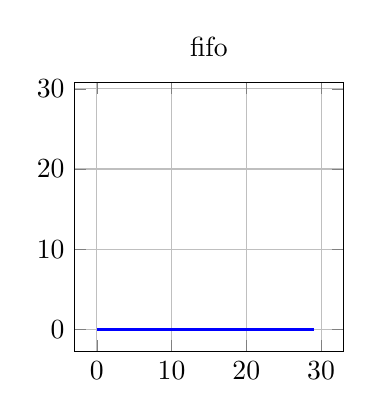
\begin{tikzpicture}
\begin{axis}[title=fifo, height=5cm, width=5cm, grid=major, xmin=({-}3.0), xmax=(33.0), ymin=({-}2.8), ymax=(30.8)]
\addplot[very thick,color=blue] coordinates {
(0,0)
(1,0)
(2,0)
(3,0)
(4,0)
(5,0)
(6,0)
(7,0)
(8,0)
(9,0)
(10,0)
(11,0)
(12,0)
(13,0)
(14,0)
(15,0)
(16,0)
(17,0)
(18,0)
(19,0)
(20,0)
(21,0)
(22,0)
(23,0)
(24,0)
(25,0)
(26,0)
(27,0)
(28,0)
(29,0)
};


\end{axis}
\end{tikzpicture}
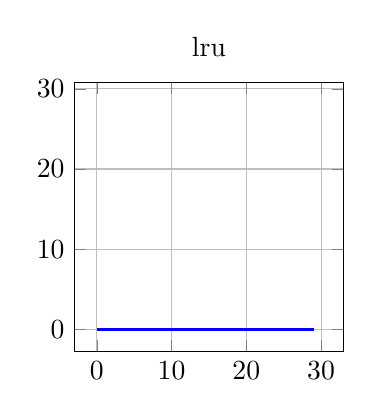
\begin{tikzpicture}
\begin{axis}[title=lru, height=5cm, width=5cm, grid=major, xmin=({-}3.0), xmax=(33.0), ymin=({-}2.8), ymax=(30.8)]
\addplot[very thick,color=blue] coordinates {
(0,0)
(1,0)
(2,0)
(3,0)
(4,0)
(5,0)
(6,0)
(7,0)
(8,0)
(9,0)
(10,0)
(11,0)
(12,0)
(13,0)
(14,0)
(15,0)
(16,0)
(17,0)
(18,0)
(19,0)
(20,0)
(21,0)
(22,0)
(23,0)
(24,0)
(25,0)
(26,0)
(27,0)
(28,0)
(29,0)
};


\end{axis}
\end{tikzpicture}
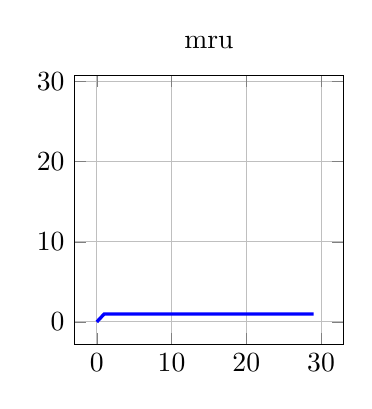
\begin{tikzpicture}
\begin{axis}[title=mru, height=5cm, width=5cm, grid=major, xmin=({-}3.0), xmax=(33.0), ymin=({-}2.8), ymax=(30.8)]
\addplot[very thick,color=blue] coordinates {
(0,0)
(1,1)
(2,1)
(3,1)
(4,1)
(5,1)
(6,1)
(7,1)
(8,1)
(9,1)
(10,1)
(11,1)
(12,1)
(13,1)
(14,1)
(15,1)
(16,1)
(17,1)
(18,1)
(19,1)
(20,1)
(21,1)
(22,1)
(23,1)
(24,1)
(25,1)
(26,1)
(27,1)
(28,1)
(29,1)
};


\end{axis}
\end{tikzpicture}
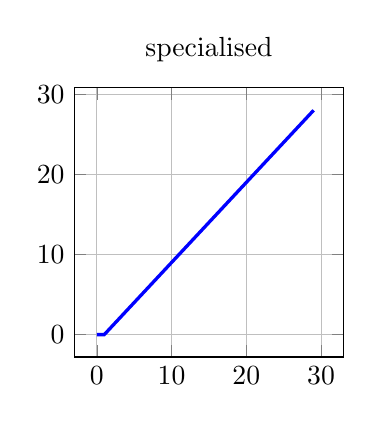
\begin{tikzpicture}
\begin{axis}[title=specialised, height=5cm, width=5cm, grid=major, xmin=({-}3.0), xmax=(33.0), ymin=({-}2.8), ymax=(30.8)]
\addplot[very thick,color=blue] coordinates {
(0,0)
(1,0)
(2,1)
(3,2)
(4,3)
(5,4)
(6,5)
(7,6)
(8,7)
(9,8)
(10,9)
(11,10)
(12,11)
(13,12)
(14,13)
(15,14)
(16,15)
(17,16)
(18,17)
(19,18)
(20,19)
(21,20)
(22,21)
(23,22)
(24,23)
(25,24)
(26,25)
(27,26)
(28,27)
(29,28)
};


\end{axis}
\end{tikzpicture}


\section{Series: math.log10(h / h + ncm + cm)}
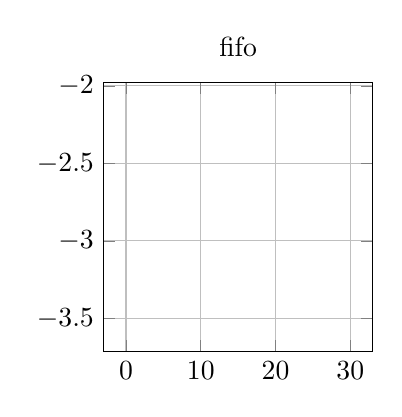
\begin{tikzpicture}
\begin{axis}[title=fifo, height=5cm, width=5cm, grid=major, xmin=({-}3.0), xmax=(33.0), ymin=({-}3.7153), ymax=({-}1.9787)]
\addplot[very thick,color=red] coordinates {
};


\end{axis}
\end{tikzpicture}
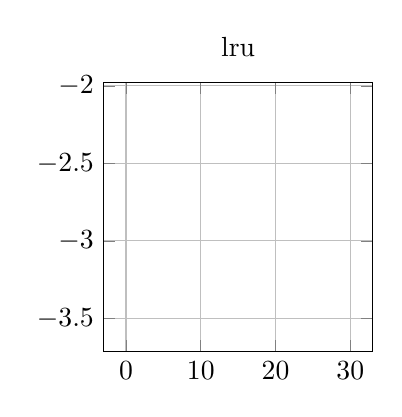
\begin{tikzpicture}
\begin{axis}[title=lru, height=5cm, width=5cm, grid=major, xmin=({-}3.0), xmax=(33.0), ymin=({-}3.7153), ymax=({-}1.9787)]
\addplot[very thick,color=red] coordinates {
};


\end{axis}
\end{tikzpicture}
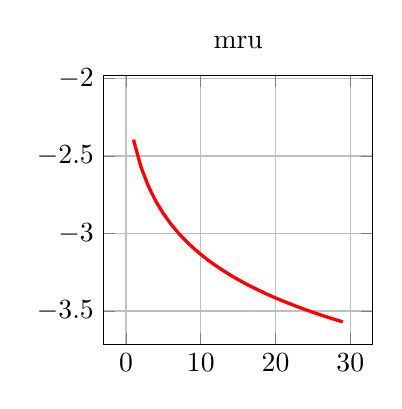
\begin{tikzpicture}
\begin{axis}[title=mru, height=5cm, width=5cm, grid=major, xmin=({-}3.0), xmax=(33.0), ymin=({-}3.7153), ymax=({-}1.9787)]
\addplot[very thick,color=red] coordinates {
(1,-2.3944516808262164)
(2,-2.5705429398818973)
(3,-2.6954816764901977)
(4,-2.792391689498254)
(5,-2.8715729355458786)
(6,-2.938519725176492)
(7,-2.9965116721541785)
(8,-3.04766419460156)
(9,-3.093421685162235)
(10,-3.13481437032046)
(11,-3.17260293120986)
(12,-3.2073650374690716)
(13,-3.239549720840473)
(14,-3.2695129442179165)
(15,-3.2975416678181597)
(16,-3.323870606540509)
(17,-3.348694190265541)
(18,-3.372175286115064)
(19,-3.3944516808262164)
(20,-3.4156409798961542)
(21,-3.4358443659844413)
(22,-3.4551495211798278)
(23,-3.473632926873841)
(24,-3.4913616938342726)
(25,-3.508395033133053)
(26,-3.5247854493212225)
(27,-3.540579716504454)
(28,-3.5558196830611912)
(29,-3.5705429398818973)
};


\end{axis}
\end{tikzpicture}
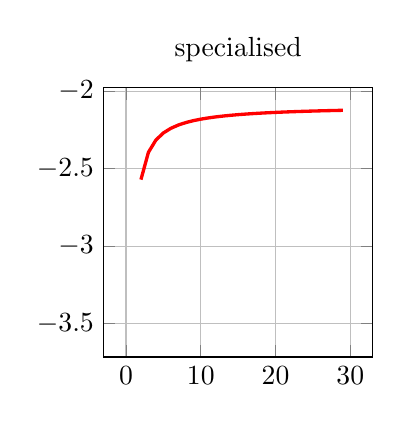
\begin{tikzpicture}
\begin{axis}[title=specialised, height=5cm, width=5cm, grid=major, xmin=({-}3.0), xmax=(33.0), ymin=({-}3.7153), ymax=({-}1.9787)]
\addplot[very thick,color=red] coordinates {
(2,-2.5705429398818973)
(3,-2.3944516808262164)
(4,-2.3152704347785913)
(5,-2.2695129442179165)
(6,-2.239549720840473)
(7,-2.218360421770535)
(8,-2.202566154587303)
(9,-2.1903316981702914)
(10,-2.1805718608811353)
(11,-2.17260293120986)
(12,-2.1659723523108467)
(13,-2.160368474792848)
(14,-2.1555695919110796)
(15,-2.151413632139922)
(16,-2.147779347484828)
(17,-2.144574207609616)
(18,-2.1417263647367903)
(19,-2.1391791757229104)
(20,-2.1368873789433254)
(21,-2.13481437032046)
(22,-2.1329302264459087)
(23,-2.131210246051635)
(24,-2.1296338578166796)
(25,-2.128183791421447)
(26,-2.1268454406491846)
(27,-2.1256063685336364)
(28,-2.124455918902204)
(29,-2.1233849085396783)
};


\end{axis}
\end{tikzpicture}


\section{Series: math.log10(h / h + ncm)}
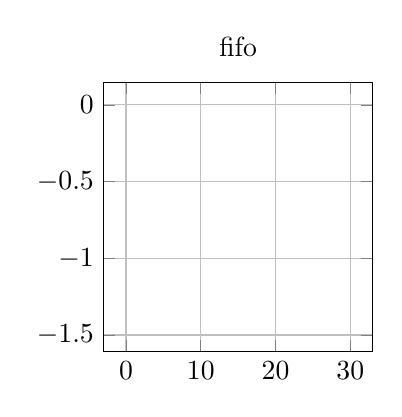
\begin{tikzpicture}
\begin{axis}[title=fifo, height=5cm, width=5cm, grid=major, xmin=({-}3.0), xmax=(33.0), ymin=({-}1.6086), ymax=(0.1462)]
\addplot[very thick,color=orange] coordinates {
};


\end{axis}
\end{tikzpicture}
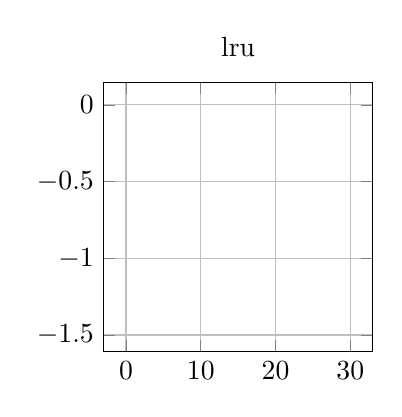
\begin{tikzpicture}
\begin{axis}[title=lru, height=5cm, width=5cm, grid=major, xmin=({-}3.0), xmax=(33.0), ymin=({-}1.6086), ymax=(0.1462)]
\addplot[very thick,color=orange] coordinates {
};


\end{axis}
\end{tikzpicture}
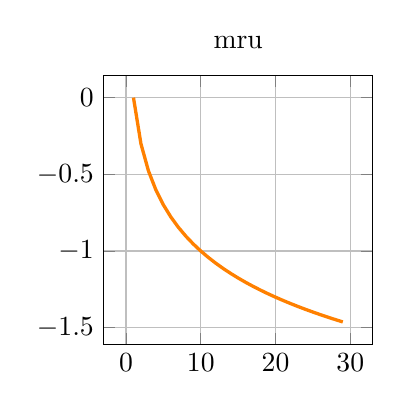
\begin{tikzpicture}
\begin{axis}[title=mru, height=5cm, width=5cm, grid=major, xmin=({-}3.0), xmax=(33.0), ymin=({-}1.6086), ymax=(0.1462)]
\addplot[very thick,color=orange] coordinates {
(1,0.0)
(2,-0.3010299956639812)
(3,-0.47712125471966244)
(4,-0.6020599913279624)
(5,-0.6989700043360187)
(6,-0.7781512503836436)
(7,-0.8450980400142568)
(8,-0.9030899869919435)
(9,-0.9542425094393249)
(10,-1.0)
(11,-1.041392685158225)
(12,-1.0791812460476249)
(13,-1.1139433523068367)
(14,-1.146128035678238)
(15,-1.1760912590556813)
(16,-1.2041199826559248)
(17,-1.2304489213782739)
(18,-1.255272505103306)
(19,-1.278753600952829)
(20,-1.3010299956639813)
(21,-1.3222192947339193)
(22,-1.3424226808222062)
(23,-1.3617278360175928)
(24,-1.3802112417116061)
(25,-1.3979400086720375)
(26,-1.414973347970818)
(27,-1.4313637641589874)
(28,-1.4471580313422192)
(29,-1.462397997898956)
};


\end{axis}
\end{tikzpicture}
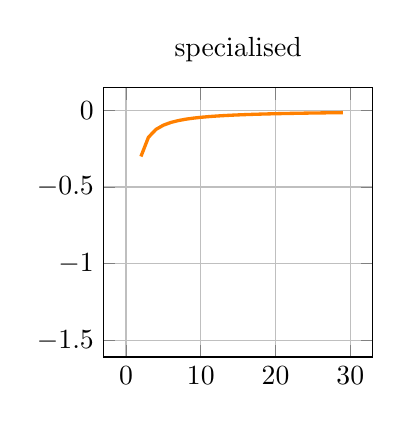
\begin{tikzpicture}
\begin{axis}[title=specialised, height=5cm, width=5cm, grid=major, xmin=({-}3.0), xmax=(33.0), ymin=({-}1.6086), ymax=(0.1462)]
\addplot[very thick,color=orange] coordinates {
(2,-0.3010299956639812)
(3,-0.17609125905568127)
(4,-0.12493873660829995)
(5,-0.09691001300805639)
(6,-0.0791812460476248)
(7,-0.06694678963061322)
(8,-0.057991946977686754)
(9,-0.05115252244738131)
(10,-0.045757490560675115)
(11,-0.04139268515822506)
(12,-0.0377885608893998)
(13,-0.03476210625921192)
(14,-0.03218468337140124)
(15,-0.02996322337744321)
(16,-0.028028723600243537)
(17,-0.026328938722349152)
(18,-0.024823583725032152)
(19,-0.023481095849522914)
(20,-0.022276394711152253)
(21,-0.021189299069938095)
(22,-0.02020338608828695)
(23,-0.01930515519538663)
(24,-0.018483405694013126)
(25,-0.017728766960431602)
(26,-0.017033339298780342)
(27,-0.01639041618816937)
(28,-0.015794267183231903)
(29,-0.015239966556736846)
};


\end{axis}
\end{tikzpicture}


\end{document}